% Options for packages loaded elsewhere
\PassOptionsToPackage{unicode}{hyperref}
\PassOptionsToPackage{hyphens}{url}
\PassOptionsToPackage{dvipsnames,svgnames,x11names}{xcolor}
%
\documentclass[
  12pt,
]{article}
\usepackage{amsmath,amssymb}
\usepackage{lmodern}
\usepackage{iftex}
\ifPDFTeX
  \usepackage[T1]{fontenc}
  \usepackage[utf8]{inputenc}
  \usepackage{textcomp} % provide euro and other symbols
\else % if luatex or xetex
  \usepackage{unicode-math}
  \defaultfontfeatures{Scale=MatchLowercase}
  \defaultfontfeatures[\rmfamily]{Ligatures=TeX,Scale=1}
\fi
% Use upquote if available, for straight quotes in verbatim environments
\IfFileExists{upquote.sty}{\usepackage{upquote}}{}
\IfFileExists{microtype.sty}{% use microtype if available
  \usepackage[]{microtype}
  \UseMicrotypeSet[protrusion]{basicmath} % disable protrusion for tt fonts
}{}
\makeatletter
\@ifundefined{KOMAClassName}{% if non-KOMA class
  \IfFileExists{parskip.sty}{%
    \usepackage{parskip}
  }{% else
    \setlength{\parindent}{0pt}
    \setlength{\parskip}{6pt plus 2pt minus 1pt}}
}{% if KOMA class
  \KOMAoptions{parskip=half}}
\makeatother
\usepackage{xcolor}
\usepackage[margin=1in]{geometry}
\usepackage{longtable,booktabs,array}
\usepackage{calc} % for calculating minipage widths
% Correct order of tables after \paragraph or \subparagraph
\usepackage{etoolbox}
\makeatletter
\patchcmd\longtable{\par}{\if@noskipsec\mbox{}\fi\par}{}{}
\makeatother
% Allow footnotes in longtable head/foot
\IfFileExists{footnotehyper.sty}{\usepackage{footnotehyper}}{\usepackage{footnote}}
\makesavenoteenv{longtable}
\usepackage{graphicx}
\makeatletter
\def\maxwidth{\ifdim\Gin@nat@width>\linewidth\linewidth\else\Gin@nat@width\fi}
\def\maxheight{\ifdim\Gin@nat@height>\textheight\textheight\else\Gin@nat@height\fi}
\makeatother
% Scale images if necessary, so that they will not overflow the page
% margins by default, and it is still possible to overwrite the defaults
% using explicit options in \includegraphics[width, height, ...]{}
\setkeys{Gin}{width=\maxwidth,height=\maxheight,keepaspectratio}
% Set default figure placement to htbp
\makeatletter
\def\fps@figure{htbp}
\makeatother
\setlength{\emergencystretch}{3em} % prevent overfull lines
\providecommand{\tightlist}{%
  \setlength{\itemsep}{0pt}\setlength{\parskip}{0pt}}
\setcounter{secnumdepth}{-\maxdimen} % remove section numbering
\usepackage[english]{babel}
\usepackage[utf8]{inputenc}
\usepackage{csquotes}
\usepackage{fancyhdr}
\usepackage{setspace}
\usepackage{geometry}
\usepackage{verbatim}
\usepackage{hyperref}
\usepackage{xcolor}
\usepackage{floatrow}
\floatsetup[table]{capposition=top}
\floatsetup[figure]{capposition=top}
\ifLuaTeX
  \usepackage{selnolig}  % disable illegal ligatures
\fi
\usepackage[backend=biber,citestyle=authoryear,maxcitenames=2,useprefix,autocite=inline,doi=false,url=false,isbn=false]{biblatex}
\addbibresource{../bibliography/nottingham-rep.bib}
\IfFileExists{bookmark.sty}{\usepackage{bookmark}}{\usepackage{hyperref}}
\IfFileExists{xurl.sty}{\usepackage{xurl}}{} % add URL line breaks if available
\urlstyle{same} % disable monospaced font for URLs
\hypersetup{
  pdftitle={Replication of @Frederiksen2022a},
  pdfauthor={Tom Brailey},
  colorlinks=true,
  linkcolor={blue},
  filecolor={Maroon},
  citecolor={Blue},
  urlcolor={Blue},
  pdfcreator={LaTeX via pandoc}}

\title{Replication of \textcite{Frederiksen2022a}}
\author{Tom Brailey\footnote{Word count: 126}}
\date{March, 2023}

\begin{document}
\maketitle

{
\hypersetup{linkcolor=}
\setcounter{tocdepth}{2}
\tableofcontents
}
\hypertarget{introduction}{%
\section{Introduction}\label{introduction}}

This memo begins by replicating the main exhibits in \textcite{Frederiksen2022a} (as well as some of the exhibits in their supplementary materials section\footnote{See \autocite{Frederiksen2022b,Frederiksen2022c}}) using the R programming language.

\hypertarget{replication}{%
\section{Replication}\label{replication}}

\hypertarget{replication-of-main-exhibits}{%
\subsection{Replication of Main Exhibits}\label{replication-of-main-exhibits}}

The main paper only contains one exhibit, Figure 1, replicated below. The figure replicates exactly, though it should be noted that the the upper panels of Figure 1 are calculated without reference to a base category, while the lower panels are the marginal means compared to the third category of the independent variable (\texttt{cancom}).

\begin{figure}
\centering
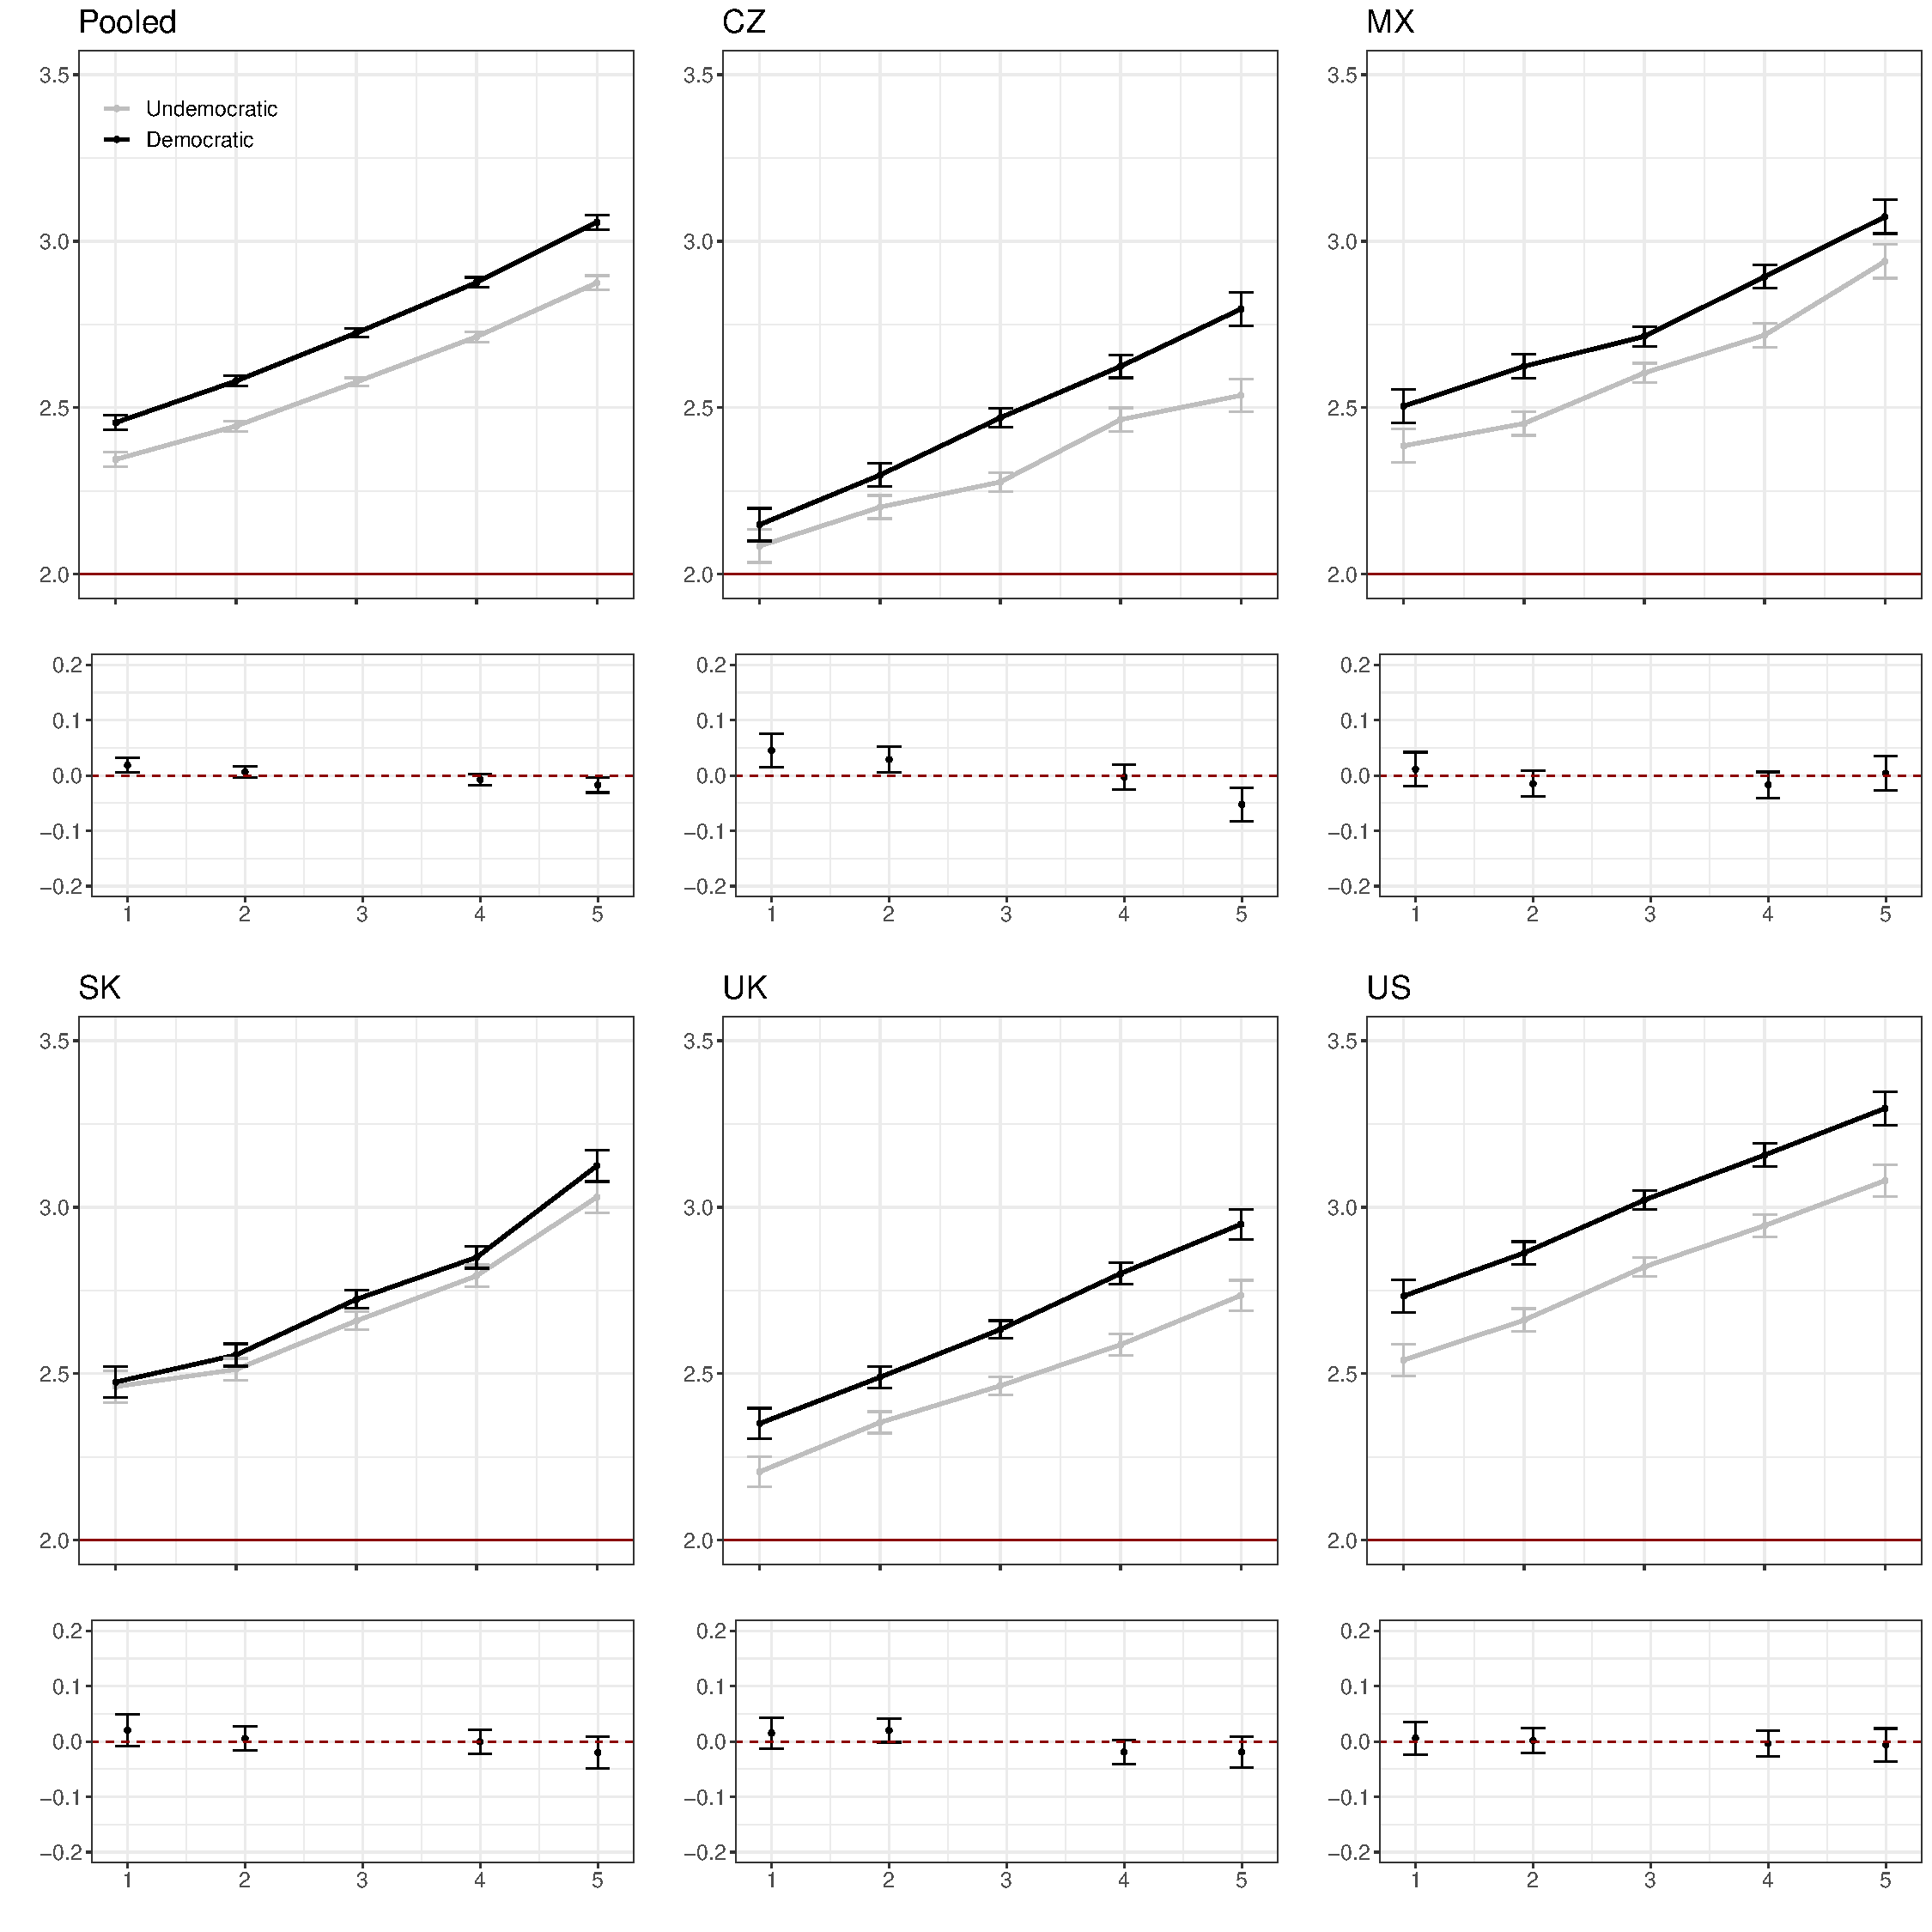
\includegraphics{../exhibits/figures/figure1_replication.pdf}
\caption{\label{fig:unnamed-chunk-1}Replication of Figure 1}
\end{figure}

\hypertarget{replication-of-appendix-a}{%
\subsection{Replication of Appendix A}\label{replication-of-appendix-a}}

Both tables in Appendix A replicate exactly in terms of point estimates, statistical significance, and number of observations.


\begin{table}[!htbp]
\caption{Average effects of undemocratic behavior andcompetence in the Czech Republic, Mexico, South Korea, the UnitedKingdom, and the United States. Candidate support is the dependentvariable in all models.}
\begin{center}
\begin{tabular}{l c c c c c}
\hline
 & Model 1 & Model 2 & Model 3 & Model 4 & Model 5 \\
\hline
Undemocratic behavior & $-0.15^{***}$ & $-0.16^{***}$ & $-0.14^{***}$ & $-0.06^{***}$ & $-0.17^{***}$ \\
                      & $(0.01)$      & $(0.01)$      & $(0.01)$      & $(0.01)$      & $(0.01)$      \\
Very incompetent      & $-0.25^{***}$ & $-0.26^{***}$ & $-0.21^{***}$ & $-0.22^{***}$ & $-0.27^{***}$ \\
                      & $(0.01)$      & $(0.02)$      & $(0.02)$      & $(0.02)$      & $(0.02)$      \\
Incompetent           & $-0.14^{***}$ & $-0.12^{***}$ & $-0.12^{***}$ & $-0.16^{***}$ & $-0.13^{***}$ \\
                      & $(0.01)$      & $(0.02)$      & $(0.02)$      & $(0.02)$      & $(0.02)$      \\
Competent             & $0.14^{***}$  & $0.17^{***}$  & $0.15^{***}$  & $0.13^{***}$  & $0.15^{***}$  \\
                      & $(0.01)$      & $(0.02)$      & $(0.02)$      & $(0.02)$      & $(0.02)$      \\
Very Competent        & $0.31^{***}$  & $0.29^{***}$  & $0.35^{***}$  & $0.39^{***}$  & $0.29^{***}$  \\
                      & $(0.01)$      & $(0.02)$      & $(0.02)$      & $(0.02)$      & $(0.02)$      \\
Constant              & $2.72^{***}$  & $2.45^{***}$  & $2.73^{***}$  & $2.72^{***}$  & $2.64^{***}$  \\
                      & $(0.01)$      & $(0.02)$      & $(0.02)$      & $(0.02)$      & $(0.02)$      \\
\hline
R$^2$                 & $0.02$        & $0.02$        & $0.02$        & $0.02$        & $0.02$        \\
Adj. R$^2$            & $0.02$        & $0.02$        & $0.02$        & $0.02$        & $0.02$        \\
Num. obs.             & $267795$      & $47221$       & $55167$       & $50002$       & $55299$       \\
RMSE                  & $1.36$        & $1.29$        & $1.43$        & $1.26$        & $1.29$        \\
N Clusters            & $14058$       & $2481$        & $2845$        & $2691$        & $2882$        \\
\hline
\multicolumn{6}{l}{\scriptsize{$^{***}p<0.001$; $^{**}p<0.01$; $^{*}p<0.05$}}
\end{tabular}
\label{table_a1}
\end{center}
\end{table}



\begin{table}[!htbp]
\caption{Table A1}
\begin{center}
\begin{tabular}{l c c c c c}
\hline
 & Model 1 & Model 2 & Model 3 & Model 4 & Model 5 \\
\hline
Undemocratic behavior           & $-0.15^{***}$ & $-0.19^{***}$ & $-0.11^{***}$ & $-0.06^{***}$ & $-0.17^{***}$ \\
                                & $(0.01)$      & $(0.02)$      & $(0.02)$      & $(0.02)$      & $(0.02)$      \\
Very incompetent                & $-0.27^{***}$ & $-0.32^{***}$ & $-0.21^{***}$ & $-0.25^{***}$ & $-0.28^{***}$ \\
                                & $(0.01)$      & $(0.03)$      & $(0.03)$      & $(0.03)$      & $(0.03)$      \\
Incompetent                     & $-0.14^{***}$ & $-0.17^{***}$ & $-0.09^{***}$ & $-0.17^{***}$ & $-0.14^{***}$ \\
                                & $(0.01)$      & $(0.02)$      & $(0.02)$      & $(0.02)$      & $(0.02)$      \\
Very competent                  & $0.15^{***}$  & $0.15^{***}$  & $0.18^{***}$  & $0.13^{***}$  & $0.17^{***}$  \\
                                & $(0.01)$      & $(0.02)$      & $(0.02)$      & $(0.02)$      & $(0.02)$      \\
Undemocratic x Very incompetent & $0.04^{*}$    & $0.13^{**}$   & $-0.01$       & $0.05$        & $0.02$        \\
                                & $(0.02)$      & $(0.04)$      & $(0.04)$      & $(0.04)$      & $(0.04)$      \\
Undemocratic x Incompetent      & $0.01$        & $0.10^{**}$   & $-0.06$       & $0.02$        & $0.03$        \\
                                & $(0.01)$      & $(0.03)$      & $(0.03)$      & $(0.03)$      & $(0.03)$      \\
Undemocratic x Competent        & $-0.02$       & $0.03$        & $-0.07^{*}$   & $0.01$        & $-0.04$       \\
                                & $(0.01)$      & $(0.03)$      & $(0.03)$      & $(0.03)$      & $(0.03)$      \\
Undemocratic x Very competent   & $-0.03$       & $-0.07$       & $-0.02$       & $-0.03$       & $-0.04$       \\
                                & $(0.02)$      & $(0.04)$      & $(0.04)$      & $(0.04)$      & $(0.04)$      \\
\hline
R$^2$                           & $0.02$        & $0.02$        & $0.02$        & $0.02$        & $0.02$        \\
Adj. R$^2$                      & $0.02$        & $0.02$        & $0.02$        & $0.02$        & $0.02$        \\
Num. obs.                       & $267795$      & $47221$       & $55167$       & $50002$       & $55299$       \\
RMSE                            & $1.36$        & $1.29$        & $1.43$        & $1.26$        & $1.29$        \\
N Clusters                      & $14058$       & $2481$        & $2845$        & $2691$        & $2882$        \\
\hline
\multicolumn{6}{l}{\scriptsize{$^{***}p<0.001$; $^{**}p<0.01$; $^{*}p<0.05$}}
\end{tabular}
\label{table:coefficients}
\end{center}
\end{table}


\hypertarget{extension}{%
\section{Extension}\label{extension}}

In this section, I extend the analysis presented in \textcite{Frederiksen2022a}.

\printbibliography

\end{document}
